
\chapter{Resultados Parciais}
\label{chap.results}

A solução foi avaliada em etapas anteriores ao desenvolvimento atual do trabalho e os resultados seguintes englobam apenas o susbsistema de \threads do \nanvix. 
\todo{Seria bom colocar um capítulo de metodologia com perguntas que gostariamos de responder e detalhamento dos experimentos}
%
Para avaliar o impacto das mudanças feitas para a virtualização, foram desenvolvidos experimentos sobre a manipulação de \threads e suporte à migração de processos no \nanvix. Todos os experimentos foram executados no processador \mppa e os resultados mostrados são valores médios de 100 replicações de cada experimento para garantir 95\% de confiança estatística, resultando em um desvio padrão inferior a 1\%.

\begin{figure}[b]
	\centering
	\subcaptionminipage[fig.fork-join]%
                   {.5\textwidth}
                   {Tempo de criação de \threads.}
                   {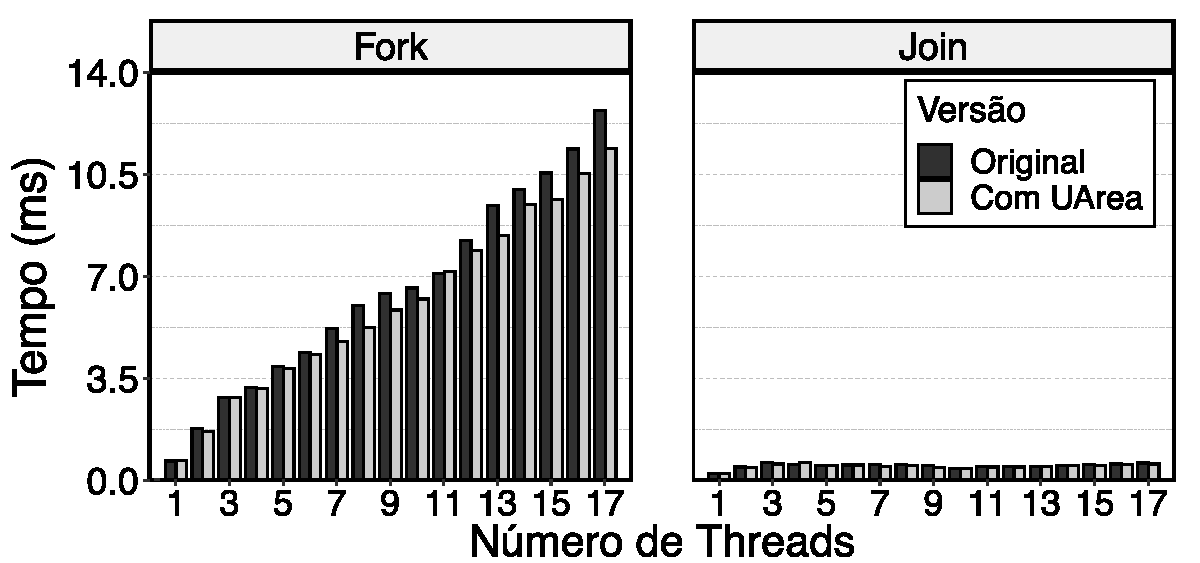
\includegraphics[width=\textwidth]{content/images/fork-join-kernel-time-bars.pdf}}
	\qquad
	\subcaptionminipage[fig.kernel-counters]
                   {.4\textwidth}
                   {Métricas do \kernel.}
                   {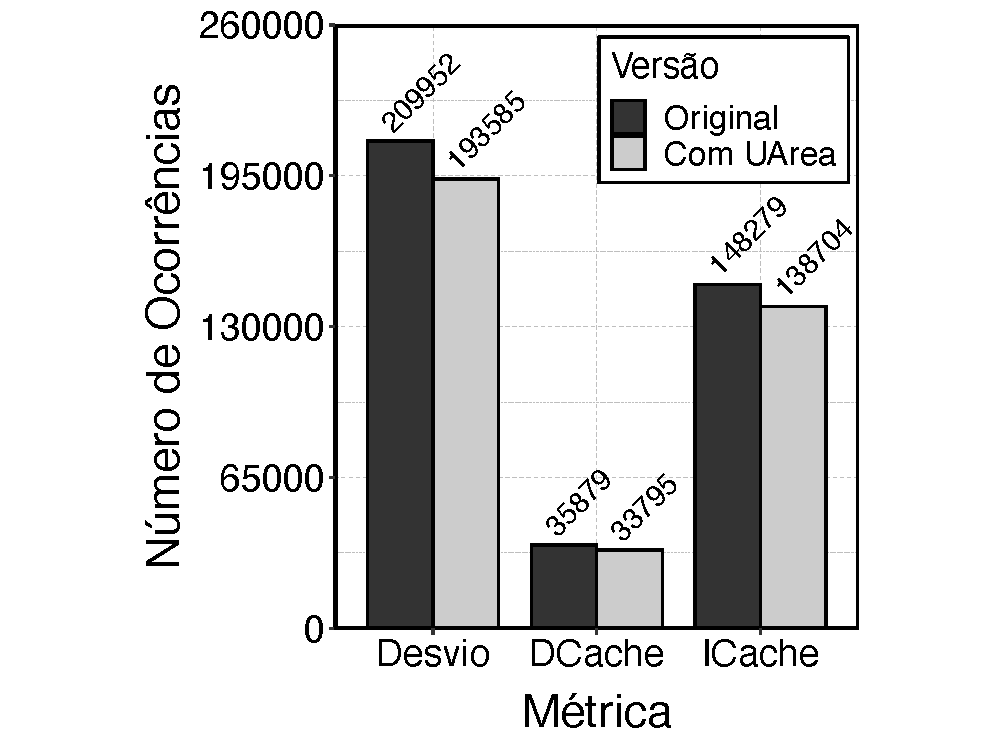
\includegraphics[width=\textwidth]{content/images/fork-join-kernel-counters.pdf}}
	\caption{Impactos da virtualização sobre a manipulação de \threads.\label{fig.threads}}%
\end{figure}

O experimento de manipulação de \threads mensura os impactos na criação e junção através de diferentes perspectivas. Especificamente, coletamos o tempo de execução, desvios e faltas ocorridas na \cache de dados e de instrução (\autoref{fig.threads}).
Os resultados apresentam um aumento no desempenho das operações de manipulação quando utilizamos a \uarea porque exploramos melhor a localidade espacial dos dados, o que, consequentemente, diminui o número de faltas na \cache.

O experimento de migração avaliou o tempo de transferência de um processo entre \clusters.
A aplicação de usuário migrada contém $352,8$~KB. Detalhadamente, foram transferidos instruções e dados ($342,8$~KB), a \uarea ($2$~KB) e uma pilha de execução ($8$~KB). O \downtime médio da aplicação, \ie o tempo que a aplicação demorou para restaurar a execução no \cluster destinatário após a migração, foi de $226$~ms. A média de tempo para o \cluster remetente enviar todos os dados foi de $218$~ms.